\chapter{लंबाई मापना}\label{ch:g2:measuring-length}

दो अलग-अलग घरों के दो दरवाज़े: इनमें से ऊँचा कौन-सा है? एक दरवाज़े को
उठाकर शहर के दूसरे छोर तक ले जाकर दूसरे के पास खड़ा नहीं किया जा
सकता। पिछले साल हमने चीज़ों की तुलना अगल-बग़ल रखकर की थी; इस साल हम
विज्ञान की सबसे बड़ी तरकीब सीखेंगे --- लंबाई को ऐसी \emph{संख्या} में
बदलना जो ख़ुद सफ़र कर सके।

\section{बिना संख्याओं के तुलना}

\begin{example}[अगल-बग़ल रखकर]\label{ex:g2:measuring-length:sidebyside}
दो पेंसिलों में से लंबी कौन-सी है, यह जानने के लिए दोनों को मेज़ पर
साथ-साथ खड़ा करो: जो बाहर निकली रह जाए वही जीती। अपनी और किसी साथी की
ऊँचाई मिलानी हो तो पीठ से पीठ लगाकर खड़े हो जाओ। यह तरीक़ा बहुत बढ़िया
चलता है --- बशर्ते दोनों चीज़ें एक जगह लाई जा सकें।
\end{example}

\begin{example}[डोरी वाली तरकीब]\label{ex:g2:measuring-length:string}
दोनों दरवाज़े मिल नहीं सकते --- पर एक डोरी दोनों के पास जा सकती है।
पहले दरवाज़े पर डोरी तानो और उसे ठीक उतनी ऊँचाई पर काट लो। अब डोरी को
दूसरे दरवाज़े तक ले जाओ: अगर डोरी छोटी पड़ जाए, तो दूसरा दरवाज़ा ऊँचा
है। डोरी पहले दरवाज़े की ऊँचाई को शहर के दूसरे छोर तक ले जाती है। एक
क़दम और आगे: क्या हो अगर हम यह ऊँचाई \emph{चिट्ठी} में भेज सकें? उसके
लिए हमें संख्याएँ चाहिए।
\end{example}

\section{क़दमों और बालिश्तों से मापना}

\begin{definition}[लंबाई मापना]\label{def:g2:measuring-length:measure}
किसी लंबाई को \emph{मापना}\index{मापना} यानी यह गिनना कि कोई चुना
हुआ \emph{मात्रक}\index{मात्रक} --- एक क़दम, एक बालिश्त, एक छोटी छड़ी
--- उस लंबाई में सिरे से सिरे तक, बिना जगह छोड़े और बिना एक-दूसरे पर
चढ़े, कितनी बार समाता है। उत्तर मात्रकों की एक संख्या होता है:
``कमरा $12$ क़दम लंबा है।''
\end{definition}

\begin{example}[इसे करके देखो: कमरा नापो]\label{ex:g2:measuring-length:pace}
अपने कमरे को एड़ी-से-पंजा जोड़कर पार करो और अपने पैरों की लंबाइयाँ
गिनो। किसी बड़े से भी यही करवाओ। हो सकता है तुम्हारी गिनती $18$ पैर
आए और बड़े की सिर्फ़ $12$ --- \emph{उसी कमरे} के लिए! किसी ने ग़लत
नहीं गिना: तुम्हारे पैर छोटे हैं, इसलिए ज़्यादा समाते हैं।
\emph{मेरे} पैर से किया गया मापन \emph{तुम्हारे} पैर से नहीं जाँचा जा
सकता।
\end{example}

\begin{omfigure}
\begin{tikzpicture}[scale=0.8]
  \draw[thick] (0,1.6) -- (9,1.6);
  \foreach \i in {0,...,11} {
    \draw[omDef, thick] (\i*0.75,1.6) rectangle ++(0.75,0.28);
  }
  \node[right, font=\small] at (9.2,1.74) {बच्चा: $12$ छोटे पैर};
  \draw[thick] (0,0) -- (9,0);
  \foreach \i in {0,...,7} {
    \draw[omThm, thick] (\i*1.125,0) rectangle ++(1.125,0.28);
  }
  \node[right, font=\small] at (9.2,0.14) {बड़ा: $8$ बड़े पैर};
\end{tikzpicture}

{\small वही दीवार, दो बार नापी गई: $12$ छोटे पैर, या $8$ बड़े पैर।
अलग पैर, अलग संख्याएँ --- दीवार तो नहीं बदली।}
\end{omfigure}

\begin{remark}[बाज़ार का झगड़ा]\label{rem:g2:measuring-length:argument}
बहुत समय तक लोग सचमुच पैरों, अँगूठों और बाँहों के फैलाव से मापते थे,
और बाज़ार झगड़ों से गूँजते थे: किसका पैर? लंबे व्यापारी का या नाटे
ग्राहक का? इसका हल, जिस पर पूरी दुनिया राज़ी हुई, यह था कि सबके लिए
\emph{एक} ही \omterm{def:g2:measuring-length:measure}{मात्रक} चुन लिया जाए --- ऐसा \omterm{def:g2:measuring-length:measure}{मात्रक} जो किसी के शरीर का न
हो।
\end{remark}

\section{सेंटीमीटर और मीटर}

\begin{definition}[सेंटीमीटर और मीटर]\label{def:g2:measuring-length:units}
\emph{सेंटीमीटर}\index{सेंटीमीटर} (लिखते हैं \unit{cm}) लंबाई का
छोटा \omterm{def:g2:measuring-length:measure}{मात्रक} है, लगभग नाख़ून की चौड़ाई जितना; वह हर रूलर पर छपा होता
है। \emph{मीटर}\index{मीटर} (लिखते हैं \unit{m}) बड़ा \omterm{def:g2:measuring-length:measure}{मात्रक} है, ठीक
$100$ सेंटीमीटर, यानी एक बहुत बड़े क़दम जितना। ये \omterm{def:g2:measuring-length:measure}{मात्रक} पृथ्वी पर
सबके लिए एक जैसे हैं: तुम्हारे \qty{20}{cm} और मेरे \qty{20}{cm}
बिलकुल बराबर हैं।
\end{definition}

\begin{omfigure}
\begin{tikzpicture}[scale=0.85]
  \draw[thick] (0,0.5) rectangle (10,1.1);
  \foreach \i in {1,...,9} {
    \draw (\i,0.5) -- (\i,0.85);
  }
  \node[below, font=\small] at (0,0.4) {$0$};
  \node[below, font=\small] at (5,0.4) {$50$};
  \node[below, font=\small] at (10,0.4) {$100$};
  \node[above, font=\small] at (5,1.35)
    {$100$ छोटे \unit{cm} मिलकर \qty{1}{m} बनाते हैं};
\end{tikzpicture}

{\small \omterm{def:g2:measuring-length:units}{मीटर} वाली छड़: एक क़तार में सौ \omterm{def:g2:measuring-length:units}{सेंटीमीटर}। निशान उन्हें एक-एक
करके गिनने के बजाय झट से गिन लेने देते हैं।}
\end{omfigure}

\begin{method}[रूलर से मापना]\label{met:g2:measuring-length:ruler}
\begin{enumerate}
  \item रूलर को वस्तु से सटाकर उसके साथ रखो;
  \item रूलर का \emph{शून्य निशान} ठीक वस्तु के एक सिरे पर रखो ---
        रूलर का किनारा नहीं, $0$ वाला निशान;
  \item दूसरे सिरे पर लिखी संख्या पढ़ो: यही लंबाई \omterm{def:g2:measuring-length:units}{सेंटीमीटर} में है।
\end{enumerate}
अगर सिरा दो निशानों के बीच पड़े, तो कहो ``\qty{7}{cm} और \qty{8}{cm}
के बीच, $8$ के ज़्यादा पास'' --- गढ़ी हुई संख्या से ईमानदार शब्द
बेहतर हैं।
\end{method}

\begin{omfigure}
\begin{tikzpicture}[scale=0.85]
  \draw[thick] (0,0) rectangle (8.4,0.7);
  \foreach \i in {0,...,12} {
    \draw (0.2+\i*0.65,0) -- (0.2+\i*0.65,0.3);
    \node[below, font=\footnotesize] at (0.2+\i*0.65,0) {\i};
  }
  \draw[thick, fill=omMeth, fill opacity=0.5]
    (0.2,1.0) rectangle (5.4,1.45);
  \node[font=\small] at (2.8,1.22) {रंगीन पेंसिल};
  \draw[dashed, omExo] (0.2,0.35) -- (0.2,1.0);
  \draw[dashed, omExo] (5.4,0.35) -- (5.4,1.0);
  \node[above, font=\small] at (5.4,1.5) {पढ़ने पर $8$: \qty{8}{cm}};
\end{tikzpicture}

{\small रूलर पढ़ना: शून्य निशान पेंसिल के एक सिरे पर, फिर दूसरा सिरा
पढ़ो। यह रंगीन पेंसिल \qty{8}{cm} लंबी है।}
\end{omfigure}

\begin{omfigure}
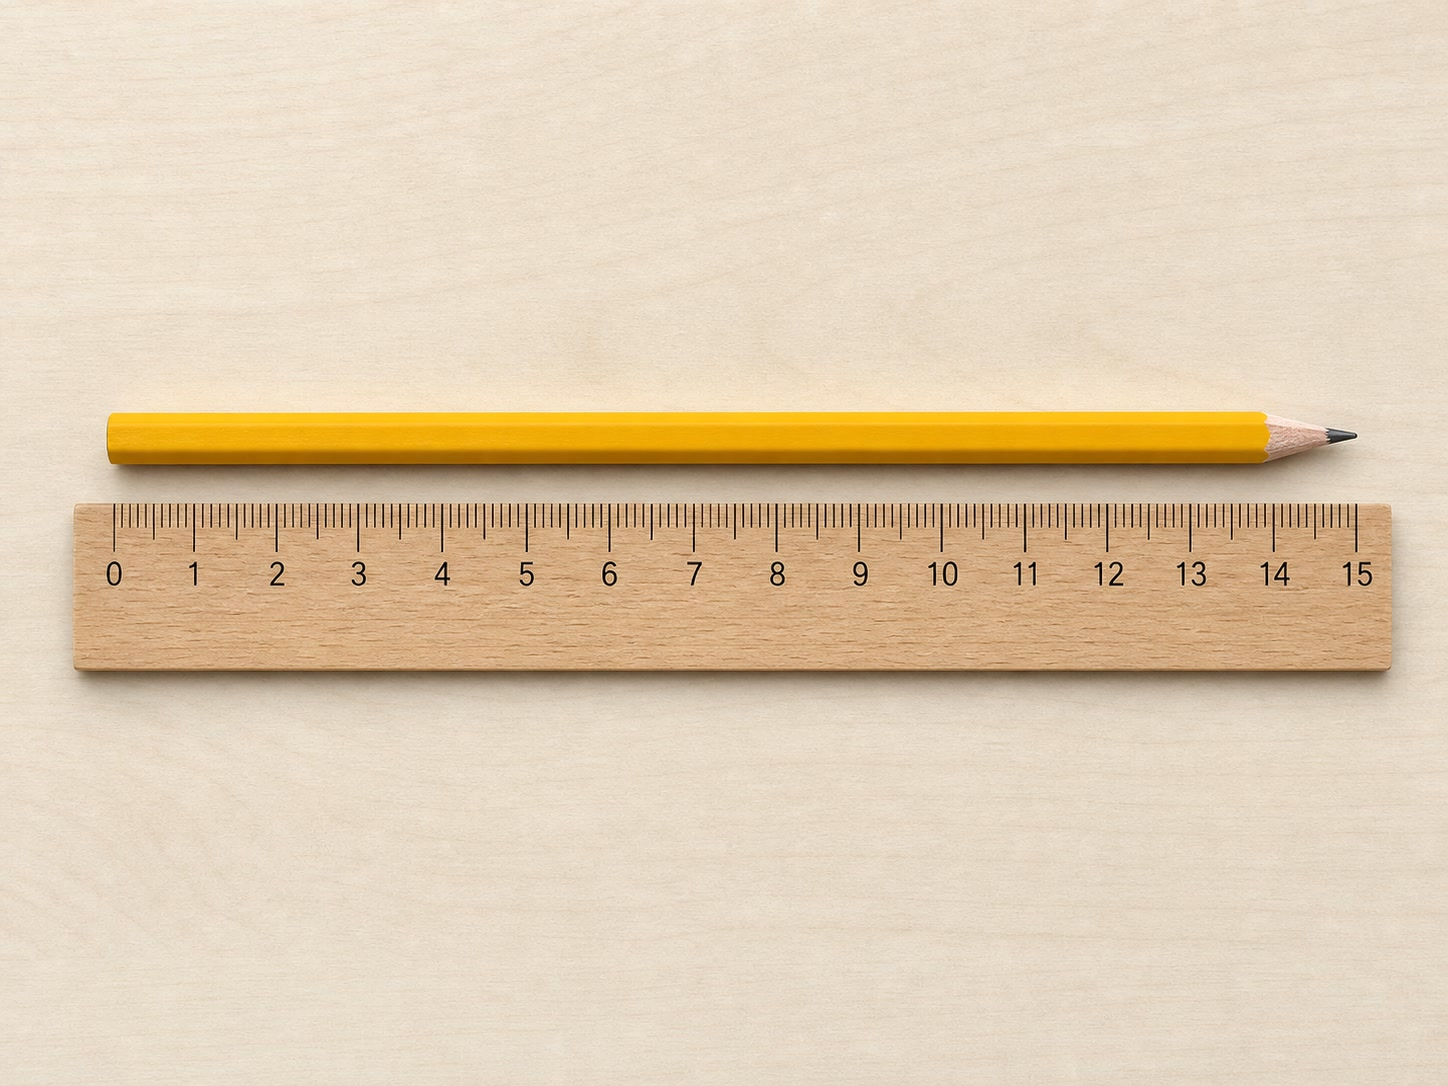
\includegraphics[width=0.52\linewidth]{images/book1/ai/g2-measuring-ruler.jpg}

{\small ठीक तरह से किया गया मापन: पेंसिल का सिरा ठीक रूलर के शून्य निशान पर बैठा है।}
\end{omfigure}

\begin{example}[किस काम के लिए कौन-सा मात्रक?]\label{ex:g2:measuring-length:whichunit}
भृंग, टिकट या अपने हाथ जैसी छोटी चीज़ें \omterm{def:g2:measuring-length:units}{सेंटीमीटर} में मापी जाती हैं।
गलियारा, बस या तरण-ताल जैसी बड़ी चीज़ें \omterm{def:g2:measuring-length:units}{मीटर} में: ताल \qty{25}{m}
लंबा है --- ज़रा सोचो, इसे नाख़ून की चौड़ाइयों में गिनना पड़ता तो!
समझदारी से \omterm{def:g2:measuring-length:measure}{मात्रक} चुन लेना मापने का आधा काम है।
\end{example}

\begin{example}[पहले अंदाज़ा, फिर जाँच]\label{ex:g2:measuring-length:estimate}
मापने से पहले खिलाड़ी अंदाज़ा लगाते हैं: रसोई की मेज़ कितनी लंबी है?
पापा कहते हैं \qty{2}{m}, लीना कहती है \qty{1}{m} और थोड़ा-सा। फिर
\omterm{def:g2:measuring-length:units}{मीटर} वाली छड़ फ़ैसला करती है: \qty{1}{m} और लगभग आधा --- लीना का
अंक। पहले अंदाज़ा लगाना आँख को सधाता है; \omterm{def:g2:measuring-length:measure}{मापना} सबको ईमानदार रखता है।
\end{example}

\section{अभ्यास}

\begin{exercise}[$\star$]\label{exo:g2:measuring-length:1}
बिना किसी रूलर के अपनी और किसी साथी की ऊँचाई की तुलना कैसे करोगे?
और उस साथी की ऊँचाई से, जो दूसरे शहर में रहता है?
\end{exercise}

\begin{exercise}[$\star$]\label{exo:g2:measuring-length:2}
मारा कक्षा को क़दमों में मापती है और $20$ पाती है; उसकी शिक्षिका $14$
पाती हैं। किसने ग़लत गिना? समझाओ।
\end{exercise}

\begin{exercise}[$\star$]\label{exo:g2:measuring-length:3}
पैर की लंबाई या बालिश्त के मुक़ाबले \omterm{def:g2:measuring-length:units}{सेंटीमीटर} में ख़ास बात क्या है?
लोग उस पर राज़ी क्यों हुए?
\end{exercise}

\begin{exercise}[$\star$]\label{exo:g2:measuring-length:4}
कौन-सा \omterm{def:g2:measuring-length:measure}{मात्रक} बेहतर बैठता है, \unit{cm} या \unit{m}: चींटी की
लंबाई; \ दरवाज़े की ऊँचाई; \ स्कूल के मैदान की लंबाई; \ इस पुस्तक की
चौड़ाई?
\end{exercise}

\begin{exercise}[$\star$]\label{exo:g2:measuring-length:5}
टिम अपने रूलर का किनारा --- शून्य निशान नहीं --- पेंसिल के सिरे से
लगाता है और \qty{13}{cm} पढ़ता है। क्या उसकी पेंसिल सचमुच
\qty{13}{cm} लंबी है? \cref{met:g2:measuring-length:ruler} की कौन-सी
बात वह भूल गया?
\end{exercise}

\begin{exercise}[$\star$]\label{exo:g2:measuring-length:6}
रूलर से मापो: अपने हाथ की चौड़ाई; \ एक चम्मच की लंबाई; \ एक मग की
ऊँचाई। हर उत्तर उसके \omterm{def:g2:measuring-length:measure}{मात्रक} के साथ लिखो।
\end{exercise}

\begin{exercise}[$\star$]\label{exo:g2:measuring-length:7}
एक दरवाज़ा \qty{2}{m} ऊँचा है। यह कितने \omterm{def:g2:measuring-length:units}{सेंटीमीटर} हुए? (याद रखो:
\qty{1}{m} यानी $100$ \unit{cm}।)
\end{exercise}

\begin{exercise}[$\star$]\label{exo:g2:measuring-length:8}
पहले अंदाज़ा लगाओ, फिर मापो: तुम्हारा बिस्तर कितने \omterm{def:g2:measuring-length:units}{मीटर} लंबा है? तुम्हारा
अंदाज़ा बहुत बड़ा था, बहुत छोटा, या लगभग सही?
\end{exercise}

\begin{exercise}[$\star\star$]\label{exo:g2:measuring-length:9}
एक रिबन \qty{45}{cm} लंबा है, दूसरा \qty{38}{cm}। कौन-सा लंबा है,
और कितने \omterm{def:g2:measuring-length:units}{सेंटीमीटर} से? क्या तुम \emph{बिना} संख्याओं के भी फ़ैसला कर
सकते थे? चिट्ठी में लिखने के लिए कौन-सा तरीक़ा आसान है?
\end{exercise}

\begin{exercise}[$\star\star$]\label{exo:g2:measuring-length:10}
दादाजी कहते हैं: ``मेरा बग़ीचा $30$ डग लंबा है।'' दादाजी को प्यार से
समझाओ कि ``$30$ डग'' को कोई दूसरा जाँच क्यों नहीं सकता, और उन्हें
इसकी जगह क्या काम में लेना चाहिए। उसी बग़ीचे को कोई छोटा बच्चा डगों
में नापे तो क्या होगा?
\end{exercise}
